%% ----------------------------------------------------------------
%% Thesis.tex -- MAIN FILE (the one that you compile with LaTeX)
%% ---------------------------------------------------------------- 

% Set up the document
\documentclass[a4paper, 11pt, oneside]{Thesis}  % Use the "Thesis" style, based on the ECS Thesis style by Steve Gunn
\graphicspath{{Figures/}}  % Location of the graphics files (set up for graphics to be in PDF format)

% Include any extra LaTeX packages required
\usepackage[square, numbers, comma, sort&compress]{natbib}  % Use the "Natbib" style for the references in the Bibliography
\usepackage{verbatim}  % Needed for the "comment" environment to make LaTeX comments
\usepackage{vector}  % Allows "\bvec{}" and "\buvec{}" for "blackboard" style bold vectors in maths
\hypersetup{urlcolor=blue, colorlinks=true}  % Colours hyperlinks in blue, but this can be distracting if there are many links.
\usepackage{setspace}


%% ----------------------------------------------------------------
\begin{document}
\frontmatter	  % Begin Roman style (i, ii, iii, iv...) page numbering

% Set up the Title Page
\title  {Direct Moving Transmitter Geolocation Based on Delay and Doppler}
\authors  {\texorpdfstring
            {\href{weiss.itamar@gmail.com}{Itamar Weiss}}
            {Itamar Weiss}
            }
\addresses  {\groupname\\\deptname\\\univname}  % Do not change this here, instead these must be set in the "Thesis.cls" file, please look through it instead
\date       {\today}
\subject    {}
\keywords   {}

\maketitle
%% ----------------------------------------------------------------

\setstretch{1.3}  % It is better to have smaller font and larger line spacing than the other way round


% Define the page headers using the FancyHdr package and set up for one-sided printing
\fancyhead{}  % Clears all page headers and footers
\rhead{\thepage}  % Sets the right side header to show the page number
\lhead{}  % Clears the left side page header

\pagestyle{fancy}  % Finally, use the "fancy" page style to implement the FancyHdr headers



%% ----------------------------------------------------------------
% The "Funny Quote Page"
\pagestyle{empty}  % No headers or footers for the following pages

\null\vfill
% Now comes the "Funny Quote", written in italics
\textit{``Write a funny quote here.''}

\begin{flushright}
If the quote is taken from someone, their name goes here
\end{flushright}

\vfill\vfill\vfill\vfill\vfill\vfill\null
\clearpage  % Funny Quote page ended, start a new page
%% ----------------------------------------------------------------

% The Abstract Page
\addtotoc{Abstract}  % Add the "Abstract" page entry to the Contents
\abstract{
\addtocontents{toc}{\vspace{1em}}  % Add a gap in the Contents, for aesthetics

We analyze the problem of geolocating a single moving transmitter using an array of
stationary receivers, and propose a one-step algorithm. Although many common methods
address this problem, they all consist of suboptimal two-step algorithms: at the first
step, several signal parameters are extracted at each receiver such as Time Of Arrival
(TOA) or Angle Of Arrival (AOA), while at the next step the extracted parameters are
used to estimate the location of the transmitter. The proposed algorithm uses the same
data used in common methods. However, it is performed in a single step by maximizing
a cost function that depends on the unknown position and velocity only. This is a natural
extension of the Direct Position Determination (DPD) algorithm for the scenario
in which the transmitter is moving in an unknown velocity. In this work, we model
the problem, present the Maximum-Likelihood (ML) cost function, explore the ML cost
function for its characteristics, suggest algorithms relevant to different scenarios, present
the Cramer-Rao lower Bound (CRB) of the problem and compare numerically the performance
of the suggested algorithms to the CRLB and to the performance of the classical
two-step methods. We show that the suggested algorithm achieves better performance
than classical methods, especially in low Signal to Noise Ratio (SNR) scenarios.

}

\clearpage  % Abstract ended, start a new page
%% ----------------------------------------------------------------

\setstretch{1.3}  % Reset the line-spacing to 1.3 for body text (if it has changed)

% The Acknowledgements page, for thanking everyone
\acknowledgements{
\addtocontents{toc}{\vspace{1em}}  % Add a gap in the Contents, for aesthetics

The acknowledgements and the people to thank go here, don't forget to include your project advisor\ldots

}
\clearpage  % End of the Acknowledgements
%% ----------------------------------------------------------------

\pagestyle{fancy}  %The page style headers have been "empty" all this time, now use the "fancy" headers as defined before to bring them back


%% ----------------------------------------------------------------
\lhead{\emph{Contents}}  % Set the left side page header to "Contents"
\tableofcontents  % Write out the Table of Contents

%% ----------------------------------------------------------------
\lhead{\emph{List of Figures}}  % Set the left side page header to "List if Figures"
\listoffigures  % Write out the List of Figures

%% ----------------------------------------------------------------
%\lhead{\emph{List of Tables}}  % Set the left side page header to "List of Tables"
%\listoftables  % Write out the List of Tables

%% ----------------------------------------------------------------
\setstretch{1.5}  % Set the line spacing to 1.5, this makes the following tables easier to read
\clearpage  % Start a new page
\lhead{\emph{Abbreviations}}  % Set the left side page header to "Abbreviations"
\listofsymbols{ll}  % Include a list of Abbreviations (a table of two columns)
{
% \textbf{Acronym} & \textbf{W}hat (it) \textbf{S}tands \textbf{F}or \\
\textbf{AOA} & \textbf{A}ngle \textbf{O}f \textbf{A}rrival \\
\textbf{CRB} & \textbf{C}ramer \textbf{R}ao lower \textbf{B}ound \\
\textbf{DD} & \textbf{D}ifferential \textbf{D}oppler \\
\textbf{DPD} & \textbf{D}irect \textbf{P}osition \textbf{D}etermination \\
\textbf{FDOA} & \textbf{F}requency \textbf{D}ifference \textbf{O}f \textbf{A}rrival \\
\textbf{FIM} & \textbf{F}ischer \textbf{I}nformation \textbf{M}atrix \\
\textbf{ML} & \textbf{M}aximum \textbf{L}ikelihood \\
\textbf{SNR} & \textbf{S}ignal to \textbf{N}oise \textbf{R}atio \\
\textbf{TDOA} & \textbf{T}ime \textbf{D}ifference \textbf{O}f \textbf{A}rrival \\
\textbf{TOA} & \textbf{T}ime \textbf{O}f \textbf{A}rrival \\
}

%% ----------------------------------------------------------------
\clearpage  %Start a new page
\lhead{\emph{Symbols}}  % Set the left side page header to "Symbols"
\listofnomenclature{lll}  % Include a list of Symbols (a three column table)
{
% symbol & name & unit \\
$L$ & the number of receivers \\
$\vec{p_\ell}$ & the position of the $\ell$-th receiver \\
$\vec{p}$ & the position of the moving transmitter \\
$\vec{v}$ & the velocity of the moving transmitter \\
$r_\ell(t)$ & the complex signal received by the $\ell$-th receiver at time $t$\\
$b_\ell$ & the complex attenuation of the signal at the $\ell$-th receiver\\
$T_\ell$ & the time delay of the signal at the $\ell$-th receiver\\
$f_\ell$ & the carrier frequency Doppler shift obseved by the $\ell$-th receiver\\
$\tilde{f}_\ell$ & the carrier frequency of the signal observed by the $\ell$-th receiver\\
$w_\ell(t)$ & the noise observed by the $\ell$-th receiver at time $t$\\
$f_c$ & the nominal carrier frequency of the transmitter\\
$\nu$ & the carrier frequency shift due to source instability of the transmitter\\
$\mu_\ell$ & the ratio between the Doppler shifted frequency and the original transmitted frequency\\
& observed by the $\ell$-th receiver\\
$\theta_\ell$ & the angle between the line connecting the transmitter and the $\ell$-th receiver and the \\
& $x$-axis\\
$\phi_\ell$ & the angle between the velocity of the transmitter and the line connecting the transmitter\\
& and the $\ell$-th receiver\\
$B$ & the signal's bandwidth\\
$c$ & the speed of light\\
$s(t)$ & the envelope of the transmitted signal at time $t$\\
$Ts$ & the time between samples\\
$T$ & the observation time interval\\
}
%% ----------------------------------------------------------------
% End of the pre-able, contents and lists of things
% Begin the Dedication page

\setstretch{1.3}  % Return the line spacing back to 1.3



\pagestyle{empty}  % Page style needs to be empty for this page
\dedicatory{For/Dedicated to/To my\ldots}

\addtocontents{toc}{\vspace{2em}}  % Add a gap in the Contents, for aesthetics


%% ----------------------------------------------------------------
\mainmatter	  % Begin normal, numeric (1,2,3...) page numbering
\pagestyle{fancy}  % Return the page headers back to the "fancy" style
\doublespacing
% Include the chapters of the thesis, as separate files
% Just uncomment the lines as you write the chapters

% Chapter 1

\chapter{Introduction and Literature Survey} % Write in your own chapter title
\label{Chapter1}
\lhead{Chapter 1. \emph{Introduction and Literature Survey}} % Write in your own chapter title to set the page header

In this work, we analyse the problem of passive geolocation of a moving transmitter, using
a stationary array of receivers. We suggest a one-step algorithm for estimating the position and velocity of the transmitter based on one sampling interval. The performance of this algorithm is analyzed, tested using Monte-Carlo simulations and compared to the performance of conventional methods.\\

The signal processing problem of passive transmitter geolocation has been greatly discussed since World War I. It has both civil and military related applications. Among the military applications we can mention passive geolocation of communication systems, radars, GPS blockers and passive low-signature geolocation of air-planes. Among the civil applications we can mention navigation. The extensive use of cellular telephony these days has increased the popularity of this field, and geolocation of cellular phone users is one of the major civil application nowadays, for focused advertising, network load monitoring and enhanced emergency services. The wireless enhanced 911 (E911) review by Zagami et al.\cite{zagami} is one example to the implementation of passive geolocation methods. The wide spread and high density of Wi-Fi networks in highly populated cities nowdays, can serve passive geolocation methods for nevigation inside buildings, or where is no GPS reception. In \cite{wifi} a method for geolocation inside buildings using the Wi-Fi signal strength is presented.\\

Unlike active localization systems such as radar or sonar, that transmit a known signal and process the signal after it was returned from the target, in passive gelocation systems the transmitted signal is usually unknown. Known signals scenarios include, for example, beacon tracking, where a system transmits a known signal in order to be tracked, and scenarios in which there is a communication system that has a known training sequence. In scenarios in which the transmitted signal is known, better performance and lower algorithm complexity can be achieved.\\

While exploring passive geolocation methods, two main approaches can be found: two-step methods and one-step methods. Many two-step methods for passive transmitter geolocation have been suggested in the past \cite {musicki,musicki_kaune_koch,torrieri, chan_jardine, chan_towers, haworth, ho_chan,ho_xu}. The two-step methods first estimate parameters characterizing the signal in each receiver, or in each pair of receivers, and then use these estimated parameters to estimate the location of the transmitter. One step methods were thoroughly discussed in literature and are considered, in general, the classical passive geolocation methods. Two step methods were very popular in the past, and also today, because the parameters characterizing the signals, such as time of arrival, frequency of arrival, signal strength etc., could have been extracted using simple analog components, and because sending the extracted parameters from all the receivers to a central processing station required low-bandwidth communication that was available in the past. Obviously, due the incomplete data used in each receiver or pair of receivers and over-parametrization, two-step methods are sub-optimal.  Recently, one-step methods \cite{dpd,dpd_nb,dop_dpd_nb,dop_dpd_wb} have been suggested and shown to have greater results than the one-step methods. The one-step methods use the sampled signals collected at each of the receivers to simultaneously estimate the position of the transmitter. High frequency digital samplers and high-bandwidth communication systems that exist today, make it possible to employ the one-step methods.\\

Although geolocation of a stationary transmitter by moving receivers has been discussed thoroughly in the literature, the problem of geolocating a moving transmitter has been less discussed. The problem of geolocating a moving transmitter shows greater complexity than geolocating a stationary transmitter, because both the position and velocity of the transmitter are unknown and need to be estimated.\\

In this work, we employ the concepts of the one-step methods for passive geolocation of a moving transmitter. \\

Along this work, we present only the two-dimensional scenario, where the position and velocity of the transmitter lie on a two-dimensional plane. It is simpler to demonstrate the principles of geolocation using the two-dimensional scenarios, and the two-dimensional scenario can be easily expanded to the three-dimensional scenario. Although many applications, such as passive air-plane geolocation, are in-fact three-dimensional scenarios, in many other applications, such as mobile phone geolocation, the plane on which the transmitter could be found is usually known.

In the following chapter, we introduce several two-step and one-step methods suggested for passive geolocation of a stationary transmitter based on delay and doppler.
The two-steps methods we introduce are TOA, TDOA, FOA and FDOA, while the one-step methods introduced are DPD and its derivatives.\\
At the last section of this chapter, we introduce the outline for our work.

\section{Two-Step Localization Methods}
\subsection{Extracting TDOA and FDOA measurements}
The first step in time and frequency shifts based two-step methods is estimating the time and frequency shifts between the received signal and another signal \cite{stein, knapp_carter}. Depending on the method, the estimation can be performed between each pair of receivers, between all the receivers and a reference receiver, or between each receiver and a known reference signal, in the case where the transmitted signal is known.\\

The ML estimation of the delay and Doppler suggested by S. Stein \cite{stein} presents the following formulation.
Two noisy signals $y_1(t)$ and $y_2(t)$, observed over the interval $(0,T)$, are assumed to contain a common signal $x(t)$, appearing in $y_2(t)$ with a relative complex gain factor $\alpha$, at a differential delay $\tau$ and with a frequency offset $\nu$, all unknown. In complex envelope notation:
\begin{eqnarray}
y_1(t) &=& x(t)+n_1(t)\\
y_2(t) &=& \alpha x(t+\tau)e^{2 \pi j \nu (t+\tau)} + n_2(t) \nonumber
\end{eqnarray}

For spectrally flat noise, the ML suggested estimator is shown to be the maximum of the complex cross-ambiguity function.
\begin{equation}
R(\tau,\nu) = \left|\frac{1}{T}\int e^{-2 \pi j f \tau} Y_1^*(f-\nu)Y_2(f)df\right|
\end{equation}
Or in the time domain:
\begin{equation}
R(\tau,\nu) = \left|\frac{1}{T}\int e^{-2 \pi j \nu (t+\tau)} y_1^*(t+\tau)y_2(t)dt\right|
\end{equation}
And in the discrete time domain:
\begin{equation}
R(\tau,\nu) = \left|\frac{1}{N} \sum_{n=0}^{N-1} e^{-2 \pi j \nu t_{n+m}} y_1^*[n+m]y_2[n]\right|
\end{equation}
Where $m=\lfloor \tau F_s \rfloor$ is the discrete time delay, $N$ is the number of samples in the interval, $t_{n+m} = \frac{1}{F_s}(n+m)$ and $F_s$ is the sampling frequency.

\subsection{TOA and TDOA Based Passive Geolocation}
In this subsection we discuss the methods to geolocate a transmitter using TOA and TDOA measurements.\\
Assuming that the TOA of the Signal-Of-Interest(SOI) to a receiver is known, the transmitter is known to be located on a circle around the receiver. \\
Adding another receiver will limit the location of the transmitter to two possible points of intersection, that using additional a-priori information about the location of the transmitter can reduce the estimation to a single position. An example for the TOA scenario can be seen in figure (\ref{fig:TOA_scenario}): Two stationary receivers are located in (-300,0) and (300,0). The estimated TOA for each receiver forms a circle of possible transmitter locations around each receiver. The two circles intersect at two points that are the two possible transmitter locations. Using a-priori information regarding the position of the transmitter, the two possible transmitter positions can be reduced to a single estimated position.\\
In the case that additional receivers are added, the spheres will not intersect in one point because of noise and errors that cause estimation errors of the TOA, and the need to use estimation methods arises.\\

TOA methods for passive geolocation are seldom used, because in order to measure the TOA, each receiver needs to know the exact time when the signal was transmitted, which is usually unknown.
Therefore, the more common methods use the TDOA measurements between pairs of receivers.\\

\begin{figure}[htbp]
\begin{center}
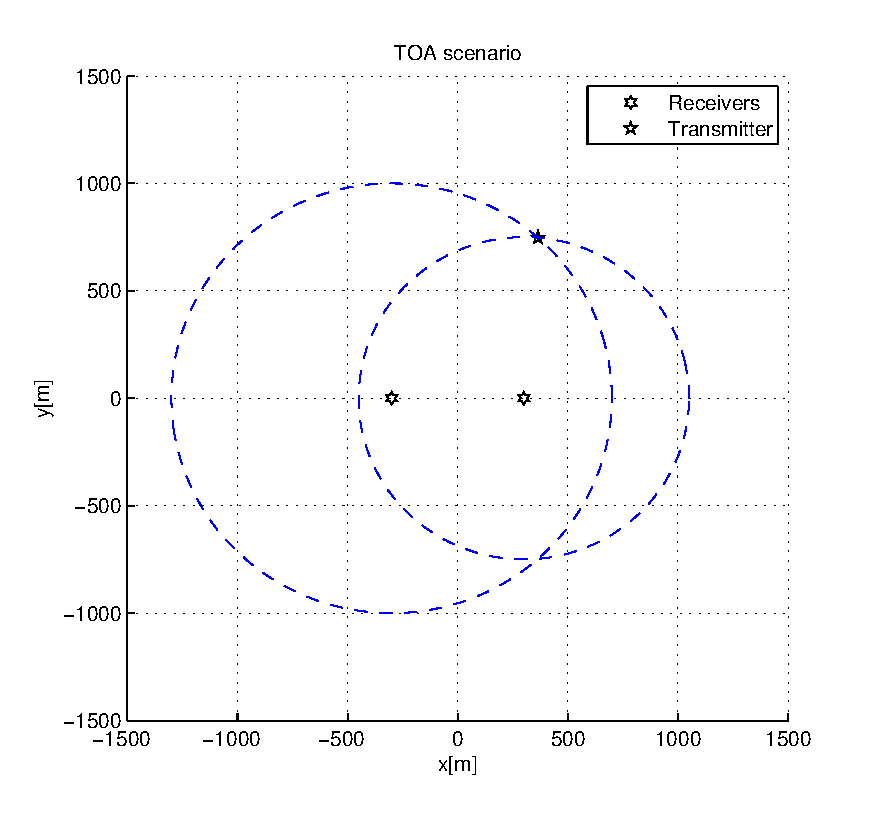
\includegraphics[scale=0.7]{TOA_scenario.eps}
\end{center}
\caption[TOA Scenario]{TOA Scenario. Two stationary receivers are located in (-300,0) and (300,0). The estimated TOA for each receiver forms a circle of possible transmitter locations around each receiver. The two circles intersect at two points that are the two possible transmitter locations. Using a-priori information regarding the position of the transmitter, the two possible transmitter positions can be reduced to a single estimated position.}
\label{fig:TOA_scenario}
\end{figure}

In TDOA based methods, each TDOA measurement locates the transmitter on a hyperbola of possible transmitter locations. At least another TDOA measurement is necessary in order to locate the transmitter at several points of intersection of the two hyperbolas. Using a-priori information about the transmitter location the several possible points can be reduced to a single solution.
Again, as additional receivers are added, the hyperboloids will not intersect in one point because of noisy measurements and errors, and the need to use estimation methods arises.
Chan and Ho \cite{chan_and_ho} suggested a simple and efficient estimator for hyperbolic location systems, and Chestnut \cite{chestnut} suggested a method for estimating the position of a stationary transmitter based on TDOA measurements and analysed its performance.\\

Figure (\ref{fig:TDOA_scenario}) shows an example of the TDOA based scenario: Two receivers are located at (-300,0) and (300,0). The TDOA measurement of this pair of receivers forms a hyperbola of possible transmitter positions. At least one more receiver is necessary in order to determine the position the transmitter.

\begin{figure}
\begin{center}
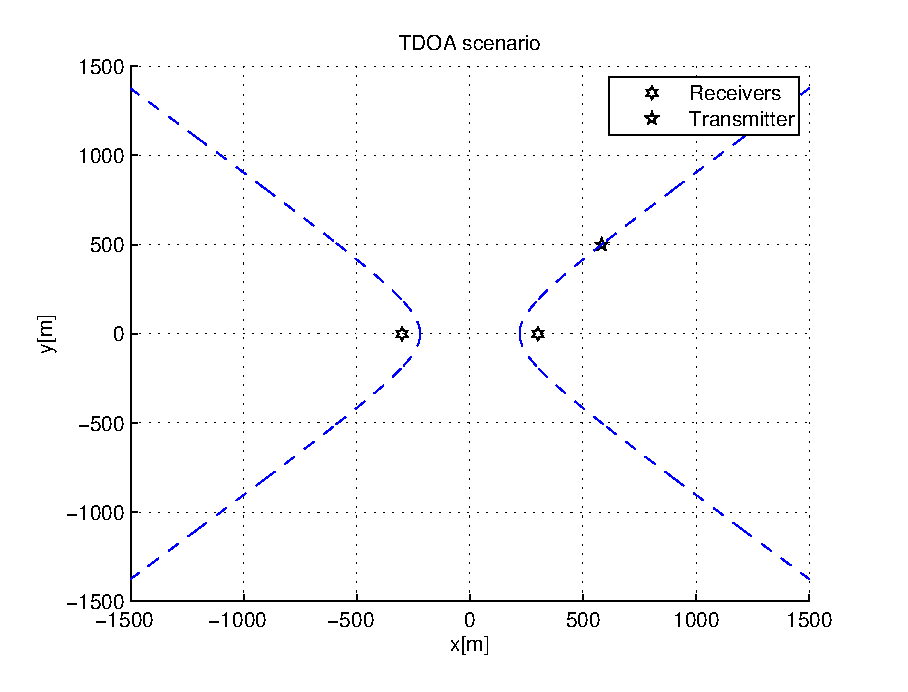
\includegraphics[scale=0.7]{TDOA_scenario.eps}
\end{center}
\caption{TDOA Scenario. Two receivers are located at (-300,0) and (300,0). The TDOA measurement of this pair of receivers forms a hyperbola of possible transmitter positions. At least one more receiver is necessary in order to determine the position the transmitter.}
\label{fig:TDOA_scenario}
\end{figure}

It is interesting to mention that the TDOA estimated in a single interval contains no information regarding the velocity of the transmitter. Thus, the velocity of the transmitter cannot be estimated using the TDOA measurements.\\

There are many suggested methods for estimating the position of a transmitter based on TDOA measurements. We will shortly introduce the application of the Weighted-Least-Squares(WLS) method, because of its relative simplicity, and only to acquire some intuition.\\

In the first step of the method introduced, the difference in the time-of-arrival is estimated for every pair of receivers, so that the matrix $\mathbf{\hat{T}}$ is estimated. The $i,j$-th element of the matrix $\mathbf{\hat{T}}$ is the time-of-arrival difference between the $i$-th and the $j$-th receivers.\\


For the transmitter position $\vec{p}$, and receivers positions $\vec{p_\ell}$, the expected $\mathbf{T(\vec{p}})$ matrix can be calculated:
\begin{equation}
T(\vec{p})_{i,j} = \frac{1}{C}\|\vec{p_i}-\vec{p}\|-\frac{1}{C}\|\vec{p_j}-\vec{p}\|
\end{equation}
The $i$,$j$-th element of $\mathbf{T(\vec{p}})$ is the expected TDOA between the $i$-th and the $j$-th receivers, if the transmitter position is $\vec{p}$.\\

A WLS TDOA cost function can then be defined as:
\begin{equation}
C_{\text{TDOA}}(\vec{p}) = \sum_{i=1}^L \sum_{j=1}^L w_{i,j}(T(\vec{p})_{i,j}-\hat{T}_{i,j})^2
\end{equation}
Where $w_{i,j}$ is the $i$,$j$-th element of the weights matrix $W$.

The WLS estimator for the position is the position $\hat{\vec{p}}$ for which the value of the WLS cost function is minimal. 
Therefore:
\begin{equation}
\hat{\vec{p}} = \text{argmin}_{\vec{p}}C_{\text{TDOA}}(\vec{p})
\end{equation}

The Known-Signals FIM related to the TOA estimation of the $\ell$-th signal is:
\begin{equation}
\text{FIM}_{\ell,\ell} = \frac{2}{\sigma_\ell^2}\left\|\frac{\partial \mathbf{m_\ell}}{\partial T_\ell}\right\|^2
\end{equation}
Where we assumed that the noise in the receivers is Gaussian i.i.d, independent between the receivers, with variance $\sigma_\ell^2$ in each receiver. The data vector $\mathbf{m_\ell}$ is the time shifted known signal, as was received in the $\ell$-th receiver if there was no noise.\\
Because $\mathbf{m_l}$ depends only on the time delay of the $\ell$-th receiver, the FIM is diagonal.
Thus:
\begin{equation}
\text{CRB}_\ell = \frac{\sigma_\ell^2}{2\left\|\frac{\partial \mathbf{m_\ell}}{\partial T_\ell}\right\|^2}
\end{equation}
So that:
\begin{equation}
\text{VAR}(\text{TOA}_\ell) \geq \frac{\sigma_\ell^2}{2\left\|\frac{\partial \mathbf{m_\ell}}{\partial T_\ell}\right\|^2}
\end{equation}
Assuming that the TOA measurements were taken using an efficient estimator, the CRB can be used to determine the weights matrix $W$.

\subsection{FOA and FDOA Based Passive Geolocation}
In the following subsection we discuss the methods to geolocate a transmitter using FOA and FDOA based methods.\\

When the transmitter is moving with a relative radial velocity to the receiver, a frequency shift of the transmitted signal is caused due to the Doppler effect.\\
Similarly to the TDOA based methods, the exact original transmitted frequency is usually unknown, and requires measurement of the FDOA between each pair of receivers.
The methods that use these measurements are sometimes also referred to as DD.\\

FOA and FDOA measurements contain information on both the position and velocity of the transmitter, unlike TDOA measurements that only contain information about the position of the transmitter. \\
Nevertheless, in order to acquire the FDOA measurements, a relative motion of the transmitter and the receivers is necessary, limiting the scenarios applicable for this method.\\

A simple, intuitive geometrical interpretation of the FDOA estimation methods is less direct, but is possible if we make a few assumptions and limit the discussion to simple scenarios. We present here two simple examples: Positioning of a stationary transmitter, transmitting a known frequency, using a moving receiver, and positioning of a stationary transmitter, transmitting an unknown frequency, using 2 moving receivers.\\

We start by describing the known transmitted frequency scenario: Consider a scenario in which the transmitter is stationary and a receiver is moving in a constant known velocity $\vec{v}$, transmitting a signal with a known frequency. The Doppler frequency shift will be proportional to the carrier frequency $F_c$ and to the relative radial velocity $\|\vec{v}\|cos\theta$, where $\theta$ is the angle between the velocity and the line connecting the transmitter and the receiver, as can be seen in figure (\ref{fig:DOP_scenario}). Because the transmitted frequency is known, the Doppler shift can be easily estimated. Since $\vec{v}$ and $F_c$ are known, $cos\theta$ can be estimated from the estimated Doppler shift, and 2 lines on which the transmitter is located are defined.\\
Additional receivers create additional lines that the transmitter lies in their spatial intersection.\\

\begin{figure}
\begin{center}
\includegraphics[scale=0.5]{DOP_scenario.eps}
\end{center}
\caption{FOA based geolocation scenario. A receiver is moving at velocity $\vec{v}$, forming an angle $\theta$ with the line connecting the positions of the receiver and the transmitter.}
\label{fig:DOP_scenario}
\end{figure}


In the case where the transmitted frequency is unknown, the Doppler shift cannot be estimated directly, and only the FDOA between pairs of receivers can be estimated. Figure (\ref{fig:FDOA_scenario}) describes a scenario in which two receivers are moving in velocities $\vec{v_1}$ and $\vec{v_2}$, forming the angles $\theta_1$ and $\theta_2$ with the lines connecting their position and the position of the transmitter. The lines connecting the position of the receivers and the position of the transmitter form the angles $\alpha_1$ and $\alpha_2$ with the $x$-axis. The FDOA between the two receivers is denoted by $\Delta f_{1,2}$.

We define the difference between the radial velocity of the receivers in relation to the transmitter by $\Delta v_{r,1,2}$ as follows:
\begin{equation}
\label{eq:Delta_v_def}
\Delta v_{r,1,2} \triangleq \|\vec{v_1}\|\text{cos}\theta_1 - \|\vec{v_2}\|\text{cos}\theta_2
\end{equation}
And then $\Delta f_{1,2}$ can be expressed as:
\begin{equation}
\label{eq:Delta_f_12}
\Delta f_{1,2}= \frac{F_c}{c} \Delta v_{r,1,2}
\end{equation}

Assuming that $\theta_2$ is known, by rearranging equation (\ref{eq:Delta_v_def}):
\begin{equation}
\label{eq:cos_theta_1}
\text{cos}\theta_1 = \frac{\Delta v_{r,1,2} + \|\vec{v_2}\|\text{cos}\theta_2}{\|\vec{v_1}\|}
\end{equation}

By rearranging equation (\ref{eq:Delta_f_12}) and substituting into (\ref{eq:cos_theta_1}) we get:
\begin{equation}
\text{cos}\theta_1 = \frac{\frac{c}{F_c}\Delta f_{1,2} + \|\vec{v_2}\|\text{cos}\theta_2}{\|\vec{v_1}\|}
\end{equation}

And so $\theta_1$ can be expressed as a function of $\theta_2$:

\begin{equation}
\label{eq:FDOA_curve}
\theta_1(\theta_2) = \text{arcos}\frac{\frac{c}{F_c}\Delta f_{1,2} + \|\vec{v_2}\|\text{cos}\theta_2}{\|\vec{v_1}\|}
\end{equation}

Equation (\ref{eq:FDOA_curve}) above describes a constant FDOA curve. The curve is defined by the known receiver velocities, and by the estimated FDOA. Every point on the curve is a possible transmitter position. Adding another receiver creates two more constant FDOA curves that the receiver lies in their intersection.

Figure (\ref{fig:FDOA_scenario_example}) shows an example of a constant FDOA curve. Two receivers are located at $(-300,0)$ and $(300,0)$ and moving with a $10[m/s]$ velocity in the positive $x$-axis direction, and the transmitter is located at $(1000,500)$.

\begin{figure}
\begin{center}
\includegraphics[scale=0.5]{FDOA_scenario.eps}
\end{center}
\caption{FDOA based geolocation scenario. Two receivers are moving in velocities $\vec{v_1}$ and $\vec{v_2}$, forming the angles $\theta_1$ and $\theta_2$ with the lines connecting their position and the position of the transmitter. The lines connecting the position of the receivers and the position of the transmitter form the angles $\alpha_1$ and $\alpha_2$ with the $x$-axis.}
\label{fig:FDOA_scenario}
\end{figure}

\begin{figure}
\begin{center}
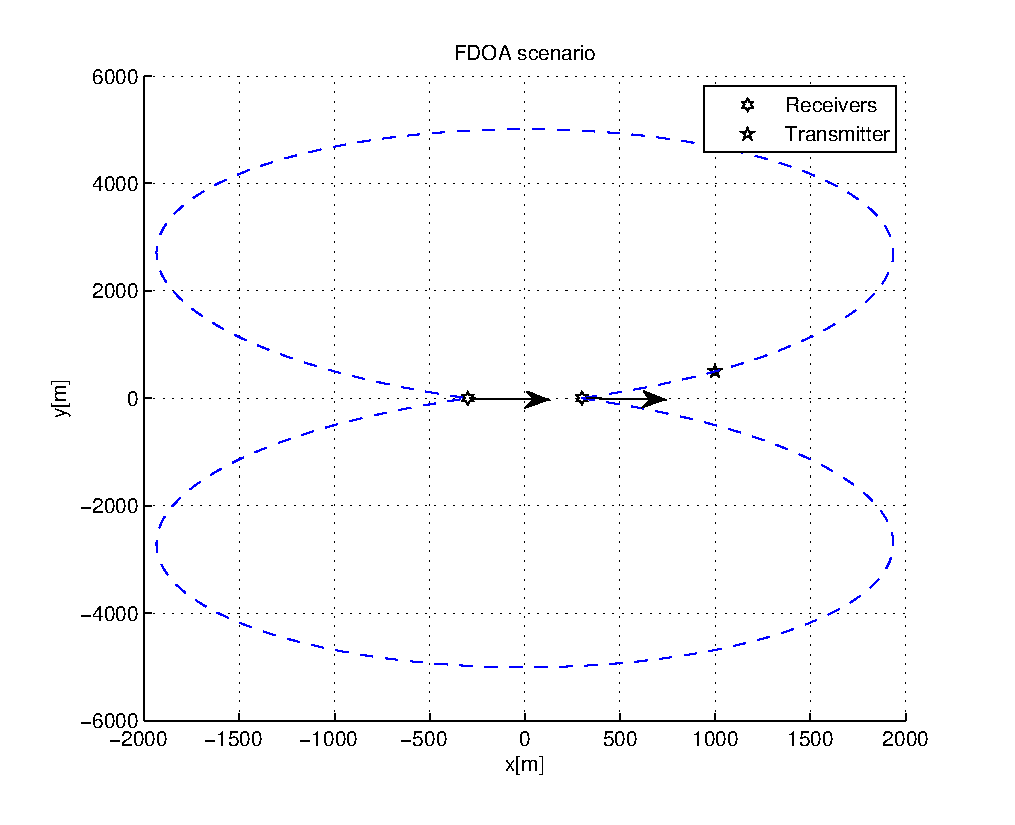
\includegraphics[scale=0.7]{FDOA_scenario_example.eps}
\end{center}
\caption{Constant FDOA curve example. Two receivers are located at $(-300,0)$ and $(300,0)$, moving with a $10[m/s]$ velocity in the positive $x$-axis direction. The transmitter is located at $(1000,500)$.}
\label{fig:FDOA_scenario_example}
\end{figure}

Just in order to acquire some understanding of FDOA based geolocation methods, we introduce a simple WLS estimation method.\\

In the first step of the method introduced, the difference in the frequency-of-arrival is estimated for every pair of receivers, so that the matrix $\hat{F}$ is estimated. The $i,j$-th element of the matrix $\hat{F}$ is the frequency-of-arrival difference between the $i$-th and the $j$-th receiver.\\

For transmitter position and velocity $(\vec{p},\vec{v})$, the expected $F(\vec{p},\vec{v})$ matrix can be calculated:
\begin{equation}
F(\vec{p},\vec{v})_{i,j} = -\frac{F_c}{c}\frac{(\vec{v}-\vec{v_i})(\vec{p}-\vec{p_i})}{|\vec{p}-\vec{p_i}|}+\frac{F_c}{c}\frac{(\vec{v}-\vec{v_j})(\vec{p}-\vec{p_j})}{|\vec{p}-\vec{p_j}|}
\end{equation}
Where $F_c$ is the carrier frequency of the signal, $c$ is the propagation speed of the signal, $\vec{v}$ is the velocity of the transmitter and $\vec{v_i}$ is the velocity of the $i$-th receiver.\\

A WLS cost function can then be defined as:

\begin{equation}
C_{\text{FDOA}}(\vec{p},\vec{v}) = \sum_{i=1}^L \sum_{j=1}^L w_{i,j}(F(\vec{p},\vec{v})_{i,j}-\hat{F}_{i,j})^2
\end{equation}

Where $w_{i,j}$ is the $i$,$j$-th element of the weight matrix $W$.
The WLS estimator for the position and velocity of the transmitter is the position and velocity that minimize the cost function:

\begin{equation}
(\hat{\vec{p}},\hat{\vec{v}}) = \text{argmin}_{(\vec{p},\vec{v})}C_{\text{FDOA}}(\vec{p},\vec{v})
\end{equation}

As opposed to the TDOA estimator, we can see that the FDOA estimate depends both on the position and on the velocity of the transmitter. Thus, both the position and velocity of the transmitter can be estimated using the FDOA measurements.\\

The Known-Signals Fischer information matrix related to the FDOA estimation of the $\ell$-th signal is:

\begin{equation}
\text{FIM}_\ell = \frac{2}{\sigma_\ell^2}\left\|\frac{\partial \mathbf{m_\ell}}{\partial f_\ell}\right\|^2
\end{equation}

Where $f_\ell$ is the frequency shift caused by the Doppler effect. We used the assumption that the noise in the receivers is Gaussian i.i.d, independent between the receivers, with variance $\sigma_\ell^2$ in each receiver. The data vector $\mathbf{m_\ell}$ is the frequency shifted known signal, as was received in the $\ell$-th receiver if there was no noise.\\
Because $\mathbf{m_l}$ depends only on the frequency shift of the $\ell$-th receiver, the FIM is diagonal.
Thus:

\begin{equation}
\text{VAR}(\text{FOA}_\ell)\geq\text{CRB}_\ell = \frac{\sigma_\ell^2}{2\left\|\frac{\partial \mathbf{m_\ell}}{\partial f_\ell}\right\|^2}
\end{equation}

Assuming that the FDOA measurements were taken using an efficient estimator, the CRB can be used to determine the weights matrix $W$.

\subsection{TDOA-FDOA Based Passive Geolocation}
\label{subsec:tdoa_fdoa}
We can easily combine the two methods suggested above using the weighted least squares (WLS) method.
If we assume that the TDOA and FDOA estimations were performed by an efficient estimator, we can use the calculated CRB for TDOA and FDOA to define the weight matrices $W_T$ and $W_F$ for the TDOA measurements and for the FDOA measurements respectively.
Then, the measurements can be combined in the following cost function:
\begin{equation}
C_{TF}(\vec{p},\vec{v}) = \sum_{i=1}^L \sum_{j=1}^L {w_T}_{i,j}(T(\vec{p})_{i,j}-\hat{T}_{i,j})^2+ {w_F}_{i,j}(F(\vec{p},\vec{v})_{i,j}-\hat{F}_{i,j})^2
\end{equation}
Where ${w_T}_{i,j}$ and ${w_F}_{i,j}$ are the $i$,$j$-th elments of the TDOA and FDOA weight matrices respectively.
The estimated position and velocity are the position and velocity that minimize the cost function:
\begin{equation}
(\hat{\vec{p}},\hat{\vec{v}}) = \text{argmin}_{(\vec{p},\vec{v})}C_{TF}(\vec{p},\vec{v})
\end{equation}

\section{DPD Algorithm Concepts}
In this section we introduce the main ideas and concepts behind the DPD algorithm \cite{dpd}.\\

Most common methods consist of two steps. The first step is to estimate a certain parameter of the
SOI, such as TDOA or FDOA. \\
The second step is to use the parameter estimated at each of the receivers, or receivers pairs, to estimate the location of the transmitter.\\
It is important to note that the estimation of the SOI parameters is done independently in each receiver or pair of receivers, so that the information used in each of the estimations is partial, consists only on the samples collected by its own antennas and does not take into consideration that all of the received signals have a common origin.\\
The DPD algorithm uses exactly the same data used in conventional methods, but it skips the first step of parameter estimation. All of the samples are collected at a central base station, and the location of the transmitter is estimated using all of the samples at once, without making any intermediate estimations.\\

The DPD algorithm advantages are mainly better performance over conventional methods using the same data and conceptual simplicity. The DPD algorithm main drawbacks are its computational complexity and the need for high band-width communication between the receivers and the central processing station in order to transfer the entire sampled signals from the receivers to the processing station.\\

The original DPD algorithm\cite{dpd} has been developed in recent years, and is now related to a family of algorithms, each of which related to a different scenario.
The original DPD algorithm \cite{dpd} assume a static scenario, in which both the transmitters and the receivers are stationary. The algorithm uses the time delays and the sensors spatial response function in order to locate multiple radio transmitters.\\

In \cite{dop_dpd_nb} a direct algorithm for the location a stationary narrow-band transmitter using an array of moving receivers is presented. The algorithm assumes that the signal is narrow band, so that the envelope of the received signal is identical in all of the receivers. The different Doppler shifts observed by the receivers are used in order to localize the transmitter. A likelihood cost function is derived, and grid-search is suggested in order to find the maximum-likelihood estimation.\\

In \cite{dop_dpd_wb} the direct algorithm is extended for locating a stationary wide-band transmitter using an array of moving receivers. This algorithm takes advantage on both the different Doppler shifts and time-delays observed by the different receivers.\\

All of the direct methods suggested above show better performance than conventional methods using the same data. The direct methods show better performance especially in low-SNR scenarios. 

In this work, we present a direct passive location algorithm for a moving transmitter using a stationary array of receivers.

\section{Outline}
\begin{itemize}
\item \textbf{Chapter 1} (this chapter) consists of an introduction to this work and of a literature survey.
\item \textbf{Chapter 2} presents the problem formulation and the derived ML estimator. The chapter handles the scenarios in which the transmitted signal is known or unknown, wide-band or narrow-band.
\item \textbf{Chapter 3} explores the characteristics of the known-signals cost function $L_2$. The function is explored in order to acquire some intuition on its behaviour, and its derivatives are developed in order to be used by gradient-based search methods.
\item \textbf{Chpater 4} suggests several possible location algorithms for different scenarios. Grid search algorithms and gradient-based algorithms are suggested. For the scenario in which the transmitter is tracked, a Kalman-filter based approach is suggested.
\item \textbf{Chapter 5} develops the known-signals Cramer-Rao lower bound of the problem.
\item \textbf{Chapter 6} presents the simulation results of several different scenarios. The results of the suggested algorithm are compared to the Cramer-Rao lower bound, and to conventional methods.
\end{itemize} % Introduction

\input{./Chapters/Chapter2} % Problem Formulation

% Chapter 1

\chapter{Exploring the cost function $L_2$} % Write in your own chapter title
\label{Chapter3}
\lhead{Chapter 3. \emph{Exploring the cost function $L_2$}} % Write in your own chapter title to set the page header

In this section, we will try to analyse the cost function $L_2$, in order to get
some insight about its behaviour. We will also develop the derivatives of $L2$ by the position and velocity in order to use them in gradient based search methods for finding its maximum.
Because $L_2$ requires the knowledge of the transmitted signal, it is mainly useful for
the case in which the transmitted signal is known.
\\
It is important to remember that given a received signal, $L_2$ is a function
of the evaluated transmitter's position and velocity estimates, meaning $L_2(\vec{p},\vec{v})$.
The dependency of the cost function in these parameters is expressed by $A_\ell$ that depends
on the relative speed and position between the transmitter and the receiver, and by $F_\ell$ that depends
on the relative distance between the transmitter and the receiver.

\section{Zero Noise Analysis - Simplified Scenario}

In order to simplify the analysis, we will use a few assumptions in the proceeding subsection.
We will assume that $b_\ell=1$ $\forall l\in\{1\dots L\}$, that there is no source instability, meaning $\nu=0$ so that $C=I$,and that the signal is narrow-band, meaning $F_\ell=I$ $\forall l\in\{1\dots L\}$.

Remembering that (from (\ref{eq:r_lWBDef})):
$$\mathbf{r_\ell}=b_\ell A_\ell F_\ell C \mathbf{s} + \mathbf{w_\ell}$$
We can write:
\begin{equation}
\mathbf{r_\ell}= A^{(0)}_\ell \mathbf{s}
\end{equation}
Where we used the assumptions that $b_\ell=1$, $C=I$, $F_\ell=I$, $\mathbf{w}_\ell=0$. $A^{(0)}_\ell$, represents the
true Doppler frequency shift caused by the relative speed of the transmitter and the emitters.

Thus:

\begin{equation}
\label{eq:simplifiedanalysis1}
(A_\ell\mathbf{s})^H\mathbf{r_\ell}=(A_\ell\mathbf{s})^H(A^{(0)}_\ell \mathbf{s})
\end{equation}

Therefore:

\begin{equation}
\|(A_\ell\mathbf{s})^H\mathbf{r_\ell}\|^2=\|(A_\ell\mathbf{s})^H(A^{(0)}_\ell \mathbf{s})\|^2=\|\mathbf{s}^H A_\ell^H A^{(0)}_\ell \mathbf{s}\|^2
\end{equation}

Defining:
\begin{equation}
D_\ell = A_\ell^H A^{(0)}_\ell
\end{equation}
Where $D_\ell$ is a frequency shift operator, shifting the signal by $f^{(0)}_\ell-f_\ell$ where $f^{(0)}_\ell$ is
the true Doppler shift of the signal received by the $\ell$-th receiver and $f_\ell$ is the expected doppler shift for a transmitter in the evaluated position and velocity $(\vec{p},\vec{v})$.\\
We can see that:

\begin{equation}
\|(A_\ell\mathbf{s})^H\mathbf{r_\ell}\|^2 = \|\mathbf{s}^H D_\ell \mathbf{s}\|^2
\end{equation}
Which is the squared absolute value of the correlation between the signal shifted by $f^{(0)}_\ell-f_\ell$ and the original signal.


\begin{equation}
L_2 = \sum_{l=1}^L \|(A_\ell\mathbf{s})^H\mathbf{r_\ell}\|^2 = \sum_{l=1}^L \|\mathbf{s}^H D_\ell \mathbf{s}\|^2
\end{equation}
Which is the sum of squared absolute value of the correlation between the signal shifted by $f^{(0)}_\ell-f_\ell$ and the original signal.
We can easily see that the maximum of the simplified $L_2$ function will occur when 
$\forall l \in \{1 \dots L \}$, $\mathbf{D_\ell}=I$, meaning that $\forall l \in \{1 \dots L \}$, 
$f_\ell = f^{(0)}_\ell$.
Notice that if the location of the receivers is known with infinite accuracy, the maximum
of the simplified cost function $L_2$ occurs at the true position of the transmitter.\\
If the there is an error in the known position of the receivers, there might not be a transmitter position and velocity ($\vec{p}, \vec{v}$) for which $\forall l \in\{1\dots L\}$, $\mathbf{D_\ell}(\vec{p},\vec{v}) = I$ and there is no guarantee that the maximum of the cost function occurs at the true transmitter position.
\\
We can notice that for the simplified scenario $\mathbf{D_\ell}(\vec{p},\vec{v})$ is actually a function of
$(\|\vec{v}\|cos\phi_\ell)$, and it can be written as $\mathbf{D_\ell}(\|\vec{v}\|cos\phi_\ell)$.


\section{Noisy Analysis - Simplified Scenario}
In this subsection we will try to analyse the effect of the noise in the receiver on the
cost function.
\\

If we consider the noise, we can write: $$ \mathbf{r_\ell}=A^{(0)}_\ell \mathbf{s}+\mathbf{w_\ell}$$

Then (\ref{eq:simplifiedanalysis1}) becomes:

\begin{equation}
(A_\ell\mathbf{s})^H\mathbf{r_\ell}=(A_\ell\mathbf{s})^H(A^{(0)}_\ell \mathbf{s}+\mathbf{w_\ell})=\mathbf{s}^H D_\ell \mathbf{s}+ \mathbf{s}^H A_\ell^H \mathbf{w_\ell}
\end{equation}

So:

\begin{eqnarray}
\label{eq:three_eight}
L_2^{(\ell)}= \\
&=& \|(A_\ell\mathbf{s})^H\mathbf{r_\ell}\|^2 = \nonumber\\ 
&=&\|\mathbf{s}^H D_\ell \mathbf{s}\|^2+\|\mathbf{s}^H A_\ell^H \mathbf{w_\ell}\|^2 + \mathbf{s}^H D_\ell \mathbf{s}(\mathbf{s}^H A_\ell^H \mathbf{w_\ell})^H + \mathbf{s}^H A_\ell^H \mathbf{w_\ell}(\mathbf{s}^H D_\ell \mathbf{s})^H = 
\nonumber \\ 
&=& \|\mathbf{s}^H D_\ell \mathbf{s}\|^2+\|\mathbf{s}^H A_\ell^H \mathbf{w_\ell}\|^2 + \mathbf{s}^H D_\ell \mathbf{s}\mathbf{w_\ell}^H A_\ell \mathbf{s} + \mathbf{s}^H A_\ell ^H \mathbf{w_\ell}\mathbf{s}^H D_\ell^H \mathbf{s} \nonumber
\end{eqnarray}

Because $\mathbf{w_\ell}$ is stochastic, $L_2$ is also a stochastic variable and we can look at its
stochastic properties such as expectation and variance.

\begin{eqnarray}
\|\mathbf{s}^H A_\ell^H \mathbf{w_\ell}\|^2 = \\
&=& \| \sum_{m=1}^N{s[m]^H a_\ell^H[m] w_\ell[m]}\|^2 = \nonumber \\
&=&\sum_{m=1}^N\sum_{n=1}^N s[m]^H s[n] a_\ell^H[m] a_\ell[n] w_\ell[m] w_\ell^H[n] \nonumber
\end{eqnarray}

Where we denoted $a_\ell[n]$ as the $n$-th element on the diagonal of $A_\ell$ and used the diagonal property of $A_\ell$.\\

Taking the expectation of the above expression we get:
\begin{eqnarray}
\label{eq:three_ten}
E\{\|\mathbf{s}^H A_\ell^H \mathbf{w_\ell}\|^2\}= \\
&=& E\left\{\sum_{m=1}^N\sum_{n=1}^N s[m]^H s[n] a_\ell^H[m] a_\ell[n] w_\ell[m] w_\ell^H[n]\right\}= \nonumber \\
&=& \sum_{m=1}^N \sigma_\ell^2 |a_\ell[m]|^2 |s[m]|^2 = \nonumber \\
&=& \sigma_\ell^2 \|\mathbf{s}\|^2 \nonumber
\end{eqnarray}

By taking the expectation of (\ref{eq:three_eight}) and substituting the result from (\ref{eq:three_ten})):
\begin{equation}
E\{L_2^{(\ell)}\}=E\{\|(A_\ell\mathbf{s})^H\mathbf{r_\ell}\|^2\}= \|\mathbf{s}^H D_\ell \mathbf{s}\|^2 + \sigma_\ell^2\|\mathbf{s}\|^2
\end{equation}
Where we used the assumptions that $\mathbf{w_\ell}$ is a zero mean, i.i.d process with $\sigma_\ell^2$ variance.\\

Thus:
\begin{eqnarray}
E\{L_2\} &=& E\{\sum_{\ell=1}^L L_2^{(\ell)}\} = \\
&=&\sum_{\ell=1}^L E\{\|(A_\ell\mathbf{s})^H\mathbf{r_\ell}\|^2\}= \sum_{\ell=1}^L \|\mathbf{s}^H D_\ell \mathbf{s}\|^2 + \sum_{\ell=1}^L \sigma_\ell^2\|\mathbf{s}\|^2 \nonumber
\end{eqnarray}

From the above result we learn that adding noise affects the expectation of the cost function by adding a constant to the cost function, that does not depend on the geometry. Thus, the maximum of the expectation of the cost function is at the same position and velocity as the cost function without any noise.

\begin{eqnarray}
\label{eq:var_l_2_l_simplified}
VAR\{L_2^{(\ell)}\} = \\
&=&VAR\{ \mathbf{s}^H D_\ell \mathbf{s}\mathbf{w_\ell}^H A_\ell \mathbf{s} + \mathbf{s}^H A_\ell^H \mathbf{w_\ell}\mathbf{s}^H D_\ell^H \mathbf{s}\} = \nonumber\\
&=&2E\{\| \mathbf{s}^H D_\ell \mathbf{s}\mathbf{w_\ell}^H A_\ell \mathbf{s} \|^2 \} + 2\Re \{E\{(\mathbf{s}^H D_\ell \mathbf{s}\mathbf{w_\ell}^H A_\ell \mathbf{s})^2 \}\} =  \nonumber \\
&=&2\| \mathbf{s}^H D_\ell \mathbf{s}\|^2\sigma_\ell^2\|\mathbf{s}\|^2 +2 \Re \left\{(\mathbf{s}^H D_\ell \mathbf{s})^2 E\left\{(\mathbf{w_\ell}^H A_\ell \mathbf{s})^2\right\}\right\} \nonumber
\end{eqnarray}

If we notice that for an arbitary complex Gaussian variable $a+bj$:
\begin{eqnarray*}
E\{(a+jb)^2\} = \\
&=& E\{a^2-b^2+2abj \}= E\{a^2\}-E\{b^2\} +2jE\{ab\}= \\
&=& \sigma^2-\sigma^2+0 = 0
\end{eqnarray*}
Where we assumed that $VAR\{a\} = VAR \{b\} = \sigma^2$ and that $a$ and $b$ have zero mean and are uncorrelated.\\
We can see that $E\left\{(\mathbf{w_\ell}^H A_\ell \mathbf{s})^2\right\}=0$  and (\ref{eq:var_l_2_l_simplified})
becomes:
\begin{equation}
VAR\{L_2^{(\ell)}\} =2\| \mathbf{s}^H D_\ell \mathbf{s}\|^2\sigma_\ell^2\|\mathbf{s}\|^2 
\end{equation}
Thus:
\begin{equation}
VAR\{L_2\} = \sum_{l=1}^L 2\| \mathbf{s}^H D_\ell \mathbf{s}\|^2\sigma_\ell^2\|\mathbf{s}\|^2 
\end{equation}
Where we used the assumption that the noise in all of the receivers is independent. Therefore, the variance of the sum becomes the sum of variances.

\section{Zero Noise Analysis - Full scenario}

In the proceeding section we will not use the assumptions used above, in the simplified scenario sections.
We will express $L_2$ using the complete signal model presented.

Remembering that (from (\ref{eq:r_lWBDef})):
 $$\mathbf{r_\ell}=b_\ell A_\ell F_\ell C \mathbf{s} + \mathbf{w_\ell}$$ 
 
 We can write:
\begin{equation}
\mathbf{r_\ell}= b_\ell A_\ell^{(0)} F_\ell^{(0)} C^{(0)} \mathbf{s}
\end{equation}
Where we used the assumption that $\mathbf{w}_\ell=0$. 
\\ \\
$A^{(0)}_\ell$, $F_\ell^{(0)}$, $C^{(0)}$ represent the true Doppler frequency shift caused by the relative speed of the transmitter and the receivers, the true delay caused by the relative distance of the transmitter and the receivers and the true transmitter frequency instability respectively.

Thus:

\begin{equation}
\label{eq:analysis1}
(A_\ell F_\ell C \mathbf{s})^H\mathbf{r_\ell}=(A_\ell F_\ell C\mathbf{s})^H(b_\ell A_\ell^{(0)} F_\ell^{(0)} C^{(0)} \mathbf{s})
\end{equation}

Therefore:

\begin{eqnarray}
\label{eq:three_eighteen}
\|(A_\ell\mathbf{s})^H\mathbf{r_\ell}\|^2 =\\
&=&\|(A_\ell F_\ell C\mathbf{s})^H(b_\ell A_\ell^{(0)} F_\ell^{(0)} C^{(0)} \mathbf{s})\|^2= \nonumber \\
&=&\|\mathbf{s}^H C^H F_\ell^H A_\ell^H b_\ell A_\ell^{(0)} F_\ell^{(0)} C^{(0)} \mathbf{s}\|^2 \nonumber
\end{eqnarray}

Defining:
\begin{equation}
D_\ell \triangleq  F_\ell^H  F_\ell^{(0)} A_\ell^H A^{(0)}_\ell C^H C^{(0)}
\end{equation}

Where $D_\ell$ is a frequency and time shift operator, shifting the signal frequency by $(f^{(0)}_\ell-f_\ell)+(\nu^{(0)}-\nu)$ and shifting the signal by $\lfloor ^{T_\ell^{(0)}}/_{T_s} \rfloor- \lfloor ^{T_\ell}/_{T_s} \rfloor$ indices. $f^{(0)}_\ell$ is the true Doppler shift of the signal received by the $\ell$-th receiver, $\nu^{(0)}$ is the true frequency instability of the transmitter and $T_\ell^{(0)}$ is the delay caused by the true distance between the transmitter and the $\ell$-the receiver.
\\
If we notice that if $A$ is a general frequency-shift matrix, $F$ is a general time shift
operator and $\mathbf{s}$ is an arbitrary signal, then $\|\mathbf{s}^H AF \mathbf{s}\|^2=\|\mathbf{s}^H FA\mathbf{s}\|^2$,
then we can write by commutating the operators in (\ref{eq:three_eighteen}):

\begin{equation}
\|(A_\ell\mathbf{s})^H\mathbf{r_\ell}\|^2 = \|b_\ell\|^2\|\mathbf{s}^H D_\ell \mathbf{s}\|^2
\end{equation}

We can see that the expression above is the correlation between the signal shifted by $\lfloor ^{T_\ell^{(0)}}/_{T_s} \rfloor- \lfloor ^{T_\ell}/_{T_s} \rfloor$ indices and by $(f^{(0)}_\ell-f_\ell)+(\nu^{(0)}-\nu)$ in frequency and the original signal.

And eventually:
\begin{equation}
\label{eq:3_21}
L_2 = \sum_{l=1}^L \|(A_\ell\mathbf{s})^H\mathbf{r_\ell}\|^2 = \sum_{l=1}^L \|\mathbf{s}^H D_\ell \mathbf{s}\|^2
\end{equation}
Which is the sum of squared absolute value of the correlation between the time and frequency shifted signal and the original signal.

\section{Noisy Analysis - Full Scenario}
In this subsection we will try to analyse the effect of the noise in the receiver on the
cost function.
\\
If we consider the noise, (\ref{eq:analysis1}) becomes:
\begin{equation}
(A_\ell F_\ell C \mathbf{s})^H\mathbf{r_\ell}=(A_\ell F_\ell C\mathbf{s})^H(b_\ell A_\ell^{(0)} F_\ell^{(0)} C^{(0)} \mathbf{s}+\mathbf{w_l}) = b_\ell \mathbf{s}^H D_\ell \mathbf{s}+ \mathbf{s}^H C^H F_\ell^H A_\ell^H \mathbf{w_\ell}
\end{equation}

So:
\begin{eqnarray}
L_2^{(\ell)}= \\
&=& \|(A_\ell F_\ell C \mathbf{s})^H\mathbf{r_\ell}\|^2 = \nonumber\\ 
&=&|b_\ell|^2\|\mathbf{s}^H D_\ell \mathbf{s}\|^2+\|\mathbf{s}^H C^H F_\ell^H A_\ell^H \mathbf{w_\ell}\|^2 + \dots \nonumber \\
\dots & +& b_\ell\mathbf{s}^H D_\ell \mathbf{s}(\mathbf{s}^H C^H F_\ell^H A_\ell^H \mathbf{w_\ell})^H + \mathbf{s}^H C^H F_\ell^H A_\ell^H \mathbf{w_\ell}(b_\ell \mathbf{s}^H D_\ell \mathbf{s})^H = 
\nonumber
\end{eqnarray}
Because $\mathbf{w_\ell}$ is stochastic, $L_2$ is also a stochastic variable and we can look at its
stochastic properties such as expectation and variance.\\

Similarly to (\ref{eq:three_ten}) we can show that:

\begin{equation}
E\{\|\mathbf{s}^H C^H F_\ell^H A_\ell^H \mathbf{w_\ell}\|^2\}= 
\sigma_\ell^2 \|\mathbf{s}\|^2 \nonumber
\end{equation}

Thus:
\begin{equation}
E\{L_2^{(\ell)}\}=E\{\|(A_\ell F_\ell C \mathbf{s})^H\mathbf{r_\ell}\|^2\}= |b_\ell|^2\|\mathbf{s}^H D_\ell \mathbf{s}\|^2 + \sigma_\ell^2\|\mathbf{s}\|^2
\end{equation}
Where we used the assumptions that $\mathbf{w_\ell}$ is a zero mean, i.i.d process with $\sigma_\ell^2$ variance.

Also, similarly to the simplified scenario, we can show that:
\begin{equation}
VAR\{L_2\} = \sum_{l=1}^L 2|b_\ell|^2\| \mathbf{s}^H D_\ell \mathbf{s}\|^2\sigma_\ell^2\|\mathbf{s}\|^2
\end{equation}


\section{Expression For $\frac{\partial L_2}{\partial v_x}$ and $\frac{\partial L_2}{\partial v_y}$}
\label{d_L2_dvx_d_vy}
In the following section, we develop the derivatives of the known signals cost function $L_2$ by the components of the velocity $v_x$ and $v_y$. This derivation allows us to perform gradient-based search in the velocity subspace for finding the maximum of the cost function.\\

Defining:
\begin{equation}
\label{eq:l2_l_def}
L_2^{(\ell)} \triangleq \|\left(A_\ell F_\ell C \mathbf{s} \right)^H\mathbf{r_\ell}\|^2
\end{equation}

The cost function $L_2$ can be expressed as:
\begin{equation}
L_2 = \sum_{l=1}^L L_2^{(\ell)}
\end{equation}

For further simplicity along the derivation we define:
\begin{equation}
\label{eq:u_l_def}
\mathbf{u_\ell} \triangleq F_\ell C \mathbf{s}
\end{equation}

By substituting (\ref{eq:u_l_def}) into (\ref{eq:l2_l_def}) we get:
\begin{equation}
L_2^{(\ell)} = \|( A_\ell \mathbf{u_\ell})^H\mathbf{r_\ell}\|^2
\end{equation}

Notice that for an arbitrary vector $\mathbf{x}$, if $y=\|\mathbf{x}\|^2=\mathbf{x}^H\mathbf{x}$ then
$$ \frac{\partial y}{\partial z} = \frac{\partial \mathbf{x}}{\partial z}^H\mathbf{x}+ \mathbf{x}^H\frac{\partial \mathbf{x}}{\partial z}=2 \Re \left\{ \frac{\partial \mathbf{x}}{\partial z}^H\mathbf{x} \right\} $$

Using the above statement for the derivative of $L_2^{(\ell)}$ by $v_x$:
\begin{equation}
\label{eq:three_thirty}
\frac{\partial}{\partial v_x} L_2^{(\ell)}  = 2 \Re
\left\{ 
\left[\frac{\partial}{\partial v_x} (Al \mathbf{u_\ell})^H \mathbf{r_\ell}\right]^H(Al \mathbf{u_\ell})^H \mathbf{r_\ell}
\right\}
\end{equation}

By using the chain rule, we can see that:
\begin{equation}
\label{eq:da_l_d_v_x}
\frac{\partial}{\partial v_x}\left( (Al \mathbf{u_\ell})^H \mathbf{r_\ell}\right) = \frac{\partial}{\partial f_\ell}\left( (Al \mathbf{u_\ell})^H \mathbf{r_\ell}\right) \frac{\partial f_\ell}{\partial v_x}
\end{equation}

We notice that:
\begin{eqnarray}
\label{eq:three_thirtytwo}
\frac{\partial}{\partial f_\ell}\left( (Al \mathbf{u_\ell})^H \mathbf{r_\ell}\right) = \\
&=& \frac{\partial}{\partial f_\ell} \left(
\sum_{n=0}^{N-1}e^{-2 \pi f_\ell T_s n}u_\ell^*[n]r_\ell[n]
\right) = \nonumber\\
&=& -2 \pi j T_s \sum_{n=0}^{N-1}ne^{-2 \pi f_\ell T_s n}u_\ell^*[n]r_\ell[n] = 
\nonumber\\
&=& -2 \pi j T_s \left( (\tilde{N} Al \mathbf{u_\ell})^H \mathbf{r_\ell}\right) \nonumber
\end{eqnarray}

Where we used the matrix $ \tilde{N}$ defined:
\begin{equation}
\tilde{N} \triangleq diag\{0,1,\dots ,N-1\}
\end{equation}

By substituting (\ref{eq:three_thirtytwo}) into (\ref{eq:da_l_d_v_x}), using the derivation of $\frac{\partial f_\ell}{\partial v_x}$ and looking at the hermitian conjugate we get:
\begin{equation}
\label{eq:three_thirtyfour}
\left[\frac{\partial}{\partial v_x} (Al \mathbf{u_\ell})^H \mathbf{r_\ell}\right]^H = -2 \pi j T_s \frac{f_c}{c}cos\theta_\ell\mathbf{r_\ell}^H(\tilde{N} A_\ell \mathbf{u_\ell})
\end{equation}

Hence, by substituting the result in (\ref{eq:three_thirtyfour}) into (\ref{eq:three_thirty}) we get:
\begin{equation}
\label{eq:three_thirtyfive}
\frac{\partial L_2}{\partial v_x} = \sum_{l=1}^L (4 \pi T_s\frac{f_c}{c} cos\theta_\ell) \Im
\left\{
(A_\ell \mathbf{u_\ell})^H \mathbf{r_\ell}\mathbf{r_\ell}^H (\tilde{N}A_\ell\mathbf{u_\ell})
\right\}
\end{equation}

And after substituting $\mathbf{u_\ell}$:
\begin{equation}
\label{eq:d_l_2_d_v_x_final}
\frac{\partial L_2}{\partial v_x} = \sum_{l=1}^L (4 \pi T_s\frac{f_c}{c} cos\theta_\ell) \Im
\left\{
(A_\ell F_\ell C \mathbf{s})^H \mathbf{r_\ell}\mathbf{r_\ell}^H (\tilde{N}A_\ell F_\ell C \mathbf{s})
\right\}
\end{equation}

And similarly:
\begin{equation}
\label{eq:d_l_2_d_v_y_final}
\frac{\partial L_2}{\partial v_y} = \sum_{l=1}^L (4 \pi T_s\frac{f_c}{c} sin\theta_\ell) \Im
\left\{
(A_\ell F_\ell C \mathbf{s})^H \mathbf{r_\ell}\mathbf{r_\ell}^H (\tilde{N}A_\ell F_\ell C \mathbf{s})
\right\}
\end{equation}

To demonstrate that the expressions above give the exact location when there is no noise, we will try to show that the derivatives of $L_2$ by the velocity components zeros for the true position of the transmitter when there is no noise.\\
For the demonstration, we take $F_\ell=I$, $C=I$ (narrow-band case, no transmitter frequency instability, for ease).

The signal received at the $\ell$-th receiver is then: 
\begin{equation}
\mathbf{r_\ell} = A_\ell^{(0)} \mathbf{s}
\end{equation}

When evaluating $A_\ell$ at the true transmitter position we get: 
\begin{equation}
A_\ell = A_\ell^{(0)}
\end{equation}

Using the above definitions, we can easily see that:
\begin{equation}
(A_\ell F_\ell C \mathbf{s})^H \mathbf{r_\ell} = \mathbf{s}^H C^{(0)H} A_\ell^{(0)H} A_\ell^{(0)} C^{(0)} \mathbf{s} = 
\|\mathbf{s}\|^2
\end{equation}

And that:
\begin{equation}
\mathbf{r_\ell}^H (\tilde{N}A_\ell F_\ell C \mathbf{s}) = 
\mathbf{s}^H C^{(0)H} A_\ell^{(0)H} \tilde{N} A_\ell^{(0)} C^{(0)} \mathbf{s} = 
\mathbf{s}^H  \tilde{N} \mathbf{s} = \sum_{n=1}^Nn\|s[n]\|^2
\end{equation}

We can clearly see that the above expressions are real. Therefore, Substituting in (\ref{eq:d_l_2_d_v_x_final}) and in (\ref{eq:d_l_2_d_v_y_final}) we can see that the true transmitter position $\vec{p_0},\vec{v_0}$ is an extremum point of the cost function:
\begin{eqnarray}
\frac{\partial L_2}{\partial v_x}|_{\vec{p_0},\vec{v_0}} = 0 \\
\frac{\partial L_2}{\partial v_y}|_{\vec{p_0},\vec{v_0}}= 0 \nonumber
\end{eqnarray}

We can also easily show that the derivative of the cost function zeros when $F_\ell \neq I$ because the
above expressions are also real.

\section{Expression For $\frac{\partial L_2}{\partial x}$ and $\frac{\partial L_2}{\partial y}$ for Narrow-Band signals}
\label{d_L2_dx_d_y_NB}
In the following section, we develop the derivatives of the known signals cost function $L_2$ by the components of the position $x$ and $y$ for the narrow-band scenario. This derivation allows us to perform gradient-based search in the position subspace for finding the maximum of the cost function.\\
We start by analysing the narrow-band scenario because the derivation and the received expressions are simpler for this scenario. In the next section we also develop these expressions for the general wide-band scenario.\\

For narrow-band signals, we assume that $F_\ell = I$, thus similarly to (\ref{eq:da_l_d_v_x}), by using the chain rule, we get:
\begin{equation}
\frac{\partial}{\partial x}\left( (Al \mathbf{u_\ell})^H \mathbf{r_\ell}\right) = \frac{\partial}{\partial f_\ell}\left( (Al \mathbf{u_\ell})^H \mathbf{r_\ell}\right) \frac{\partial f_\ell}{\partial x}
\end{equation}

Using the result of (\ref{eq:three_thirtytwo}) and the expression for $\frac{\partial f_\ell}{\partial x}$ we get:

\begin{equation}
\frac{\partial}{\partial x}((A_\ell \mathbf{u_\ell})^H \mathbf{r_\ell}) = - 2 \pi j T_s ((\tilde{N} A_\ell \mathbf{u_\ell})^H\mathbf{r_\ell})\frac{f_c}{c}\frac{\|\vec{v}\|}{d_\ell} \sin \phi_\ell \sin \theta_\ell
\end{equation}

Therefore, similarly to (\ref{eq:three_thirtyfive}):

\begin{equation}
\frac{\partial L_2}{\partial x} = -\sum_{l=1}^L (4 \pi T_s \frac{f_c}{c}\frac{\|\vec{v}\|}{d_\ell}\sin \phi_\ell \sin \theta_\ell ) \Im
\left\{
(A_\ell C \mathbf{s_\ell})^H \mathbf{r_\ell}\mathbf{r_\ell}^H (\tilde{N}A_\ell C \mathbf{s_\ell})
\right\}
\end{equation}

And similarly:
\begin{equation}
\frac{\partial L_2}{\partial y} = \sum_{l=1}^L (4 \pi T_s \frac{f_c}{c}\frac{\|\vec{v}\|}{d_\ell}\sin \phi_\ell \cos \theta_\ell ) \Im
\left\{
(A_\ell C \mathbf{s_\ell})^H \mathbf{r_\ell}\mathbf{r_\ell}^H (\tilde{N}A_\ell C \mathbf{s_\ell})
\right\}
\end{equation}
To demonstrate that when there is no noise, there is an extremum point in the true position of the transmitter, we can see that the expression inside the $\Im\{\dots\}$ operator is identical to the one in the expression for $\frac{\partial L_2}{\partial v_x}$. So, for the true position of the transmitter, the
expression inside the $\Im\{\dots\}$ operator is real, and we get:
\begin{eqnarray}
\frac{\partial L_2}{\partial x}|_{\vec{p_0},\vec{v_0}} = 0 \\
\frac{\partial L_2}{\partial y}|_{\vec{p_0},\vec{v_0}}= 0 \nonumber
\end{eqnarray}

\section{Expression For $\frac{\partial L_2}{\partial x}$ and $\frac{\partial L_2}{\partial y}$ for Wide-Band signals}
\label{d_L2_dx_dy_WB}
In the following section, we develop the derivatives of the known signals cost function $L_2$ by the components of the position $x$ and $y$ for the general wide-band scenario. This derivation allows us to perform gradient-based search in the position subspace for finding the maximum of the cost function.\\

In order to derive an expression for $\frac{\partial L_2}{\partial x}$ and $\frac{\partial L_2}{\partial y}$ for wide-band signals, we can relate to $F_\ell$ as a continuous time-shift operator.\\

We can write:
\begin{equation}
L_2^{(\ell)}=\|(A_\ell F_\ell C\mathbf{s})^H\mathbf{r_\ell}\|^2 = \|(A_\ell C F_\ell \mathbf{s})^H\mathbf{r_\ell}\|^2= \|(A_\ell C \mathbf{s_\ell})^H\mathbf{r_\ell}\|^2
\end{equation}

Where we denote:
\begin{equation}
\mathbf{s_\ell} \triangleq [s(t_1-T_\ell) \dots s(t_N-T_\ell)]^T                                                           
\end{equation}

By using the chain rule, we know that:
\begin{equation}
\label{eq:d_l_2_d_x}
\frac{\partial L_2}{\partial x} = \sum_{l=1}^L \frac{\partial L_2^{(\ell)}}{\partial x}=\sum_{l=1}^L \frac{\partial L_2^{(\ell)}}{\partial T_\ell}\frac{\partial T_\ell}{\partial x}+\frac{\partial L_2^{(\ell)}}{\partial f_\ell}\frac{\partial f_\ell}{\partial x}
\end{equation}

Looking at:

\begin{equation}
\frac{\partial L_2^{(\ell)}}{\partial T_\ell} = \frac{\partial}{\partial T_\ell} \|(A_\ell C \mathbf{s_\ell})^H\mathbf{r_\ell}\|^2
\end{equation}

We notice that:
\begin{equation}
\frac{\partial}{\partial T_\ell} (Al C \mathbf{s_\ell})^H \mathbf{r_\ell} = - (Al C \mathbf{\dot{s_\ell}})^H \mathbf{r_\ell}
\end{equation}

Thus:
\begin{eqnarray}
\frac{\partial L_2^{(\ell)}}{\partial T_\ell} = \\
&=& 2 \Re \{(- (Al C \mathbf{\dot{s_\ell}})^H \mathbf{r_\ell})^H (Al C \mathbf{s_\ell})^H \mathbf{r_\ell} \} \nonumber\\
&=& -2 \Re \{(Al C \mathbf{s_\ell})^H \mathbf{r_\ell} \mathbf{r_\ell}^H (A_\ell C \mathbf{\dot{s_\ell}})\} \nonumber
\end{eqnarray}

Subtituting the expressions for $\frac{\partial L_2^{(\ell)}}{\partial T_\ell}$, $\frac{\partial L_2^{(\ell)}}{\partial f_\ell}$, $\frac{\partial T_\ell}{\partial x}$ and $\frac{\partial f_\ell}{\partial x}$ into (\ref{eq:d_l_2_d_x}) we get:
\begin{eqnarray}
\frac{\partial L_2}{\partial x} = \\
&=& \sum_{l=1}^L -2 \Re \left\{ (A_\ell C \mathbf{s_\ell})^H \mathbf{r_\ell} \mathbf{r_\ell}^H (A_\ell C \mathbf{\dot{s_\ell}})\right\}\frac{1}{c}\cos\theta_\ell - \nonumber \\
&-& 4\pi T_s \frac{F_c}{c} \frac{\|\vec{v}\|}{d_\ell} \sin \phi_\ell \sin \theta_\ell \Im \left\{ (A_\ell C  \mathbf{s_\ell})^H \mathbf{r_\ell} \mathbf{r_\ell}^H (\tilde{N} A_\ell C \mathbf{s_\ell})\right\} \nonumber
\end{eqnarray}

And similarly for $\frac{\partial L_2}{\partial y}$:
\begin{eqnarray}
\frac{\partial L_2}{\partial y} = \\
&=& \sum_{l=1}^L -2 \Re \left\{ (A_\ell C \mathbf{s_\ell})^H \mathbf{r_\ell} \mathbf{r_\ell}^H (A_\ell C \mathbf{\dot{s_\ell}})\right\}\frac{1}{c}\sin\theta_\ell + \nonumber \\
&+& 4\pi T_s \frac{F_c}{c} \frac{\|\vec{v}\|}{d_\ell} \sin \phi_\ell \cos \theta_\ell \Im \left\{ (A_\ell C  \mathbf{s_\ell})^H \mathbf{r_\ell} \mathbf{r_\ell}^H (\tilde{N} A_\ell C \mathbf{s_\ell})\right\} \nonumber
\end{eqnarray}

And now we can go ahead and use these expressions in order to preform a gradient-based search in the position subspace for the maximum of the cost-function.

\section{Peak Size Approximation}
As we saw before, the one-step cost function is not necessarily convex, and is usually not convex outside the area of its maximum. Only in a small area around the maximum, whose dimensions vary from scenario to scenario, the cost function is convex, and all of the gradient based methods that introduce lower computational complexity than grid search based methods could be used. 

In fact, in the scenario where there is no a priori information regarding the location of the transmitter, and the search area is wide, a proposed method would be to perform a rough grid search, up to the resolution of the peak size, and then perform a fine gradient-based search to find the location of the peak in high accuracy and in low-complexity.

It is rather complicated to deduce a general expression for the size of the peak, since it depends on the exact transmitted signal and on the scenario's geometry, but by following a few simplifying assumptions we are able to derive a rough approximation of the peak's magnitude.

The first assumption that we make, is regarding the ambiguity function of the transmitted signal. We assume that the ambiguity function of the signal has a peak with a width of $\delta t$ in time and $\delta f$ in frequency, as can be seen in figure (add a figure). Although the ambiguity function of most signals is not actually bounded in time or frequency, we are usually able to determine an estimate of the magnitude of the ambiguity function's peak size - an area that contains most of the "energy" of the ambiguity function. As we saw in (\ref{eq:3_21}) $L_2$ is a superposition of the $L_2^{(\ell)}$ cost functions generated by each of the receivers. Each one of the $L_2^{(\ell)}$ cost functions is actually a mapping between the ambiguity function, and the estimated position and velocity of the transmitter. The value of the cost function in each point in position and velocity space is the value of the ambiguity function for the difference in time and frequency between the time and frequency shift for the real position and velocity of the transmitter, and the time and frequency shift for the estimated position and velocity of the transmitter, as can be seen here:

\begin{equation}
\label{eq:delta_t_def}
\delta t = \frac{\sqrt{(x-x_0)^2+(y-y_0)^2}}{C}-\frac{\sqrt{(x-x_r)^2+(y-y_r)^2}}{C}
\end{equation}

\begin{equation}
\label{eq:delta_f_def}
\delta f = -\frac{f_c}{C} \frac{\vec{v_0} (\vec{p_0}-\vec{p_r})}{\|\vec{p_0}-\vec{p_r}\|}+
\frac{f_c}{C} \frac{\vec{v} (\vec{p}-\vec{p_r})}{\|\vec{p}-\vec{p_r}\|}
\end{equation}

where $x_0$,$y_0$,$\vec{p_0}$,$\vec{v_0}$ represent the real position and velocity of the transmitter, and $x_r$,$y_r$,$\vec{p_r}$ represent the position of the $\ell$-th receiver.

From (\ref{eq:delta_t_def}) we notice that every $\delta t$ in the ambiguity function translates to a circle in the position space around the receiver, with a radius of $C(t_0+\delta t)$, where $t_0$ is the real time delay of the received signal. 
Thus, a peak of the ambiguity function with a $\delta t$ width would be found on a circular strip with a width of $C\delta t$ as can be seen in figure (add figure).

From (\ref{eq:delta_f_def}) we notice that every $\delta f$ translates to a line that originates in the position of the receiver, since every $\delta f$ determines a value for $\vec{v} (\vec{p}-\vec{p_r})$.
Thus, a peak of the ambiguity function with a $\delta f$ width would be found on a sector with an origin in the position of the receiver.
In order to derive an approximate expression of the width of the sector in the area of the peak in the position space, we can use the expressions for the derivatives of $f_\ell$ in $x$ and in $y$ to perform a first order approximation.

We know that:
\begin{eqnarray}
\frac{\partial f_\ell}{\partial x} &=& \frac{f_c}{C} \frac{\|\vec{v_0}\|}{d_\ell} \sin \phi_\ell\sin \theta_\ell \nonumber \\
\frac{\partial f_\ell}{\partial y} &=& -\frac{f_c}{C} \frac{\|\vec{v_0}\|}{d_\ell} \sin \phi_\ell \cos \theta_\ell  \nonumber
\end{eqnarray}

Assuming the the distance from the receiver is much larger the the width of the peak we can assume that $\phi_\ell$ and $\theta_\ell$ are constant, and then for a tangent change in position $\delta l$ we get a frequency shift of:
\begin{equation}
\delta f = \frac{f_c}{C} \frac{\|\vec{v_0}\|}{d_\ell} \sin\phi_\ell \delta l
\end{equation}

To summarize, as can be seen in figure (add figure), we can approximate the width of the peak in the position space in the radial and tangent directions by:
\begin{eqnarray}
\delta r &=& C \delta t \nonumber \\
\delta l &=& \frac{C}{f_c} \frac{d_\ell}{\|\vec{v_0}\|}\frac{1}{\sin \phi_\ell} \delta f \nonumber
\end{eqnarray}

Of course, what we have developed so far only relates to the cost function for an individual receiver $L_2^{(\ell)}$. It has to be taken into consideration that the $L_2$ cost function is a super position of all the individual $L_2^{(\ell)}$ cost functions.

In the velocity space, all the points with the same $\|\vec{v}\| \cos \theta_\ell$ have the same Doppler shift. Thus, as can be seen in figure (add figure), an ambiguity function peak with a width of $\delta f$ would be translated to a strip with a radial width of $\delta \|\vec{v}\| = \frac{f_C}{C}\delta f$.

Similarly to the position space, since the $L_2$ cost function is a super position of all of the individual $L_2^{(\ell)}$ cost functions, the width of the peak would be determined by the geometry of the particular scenario. Assuming that the receivers are evenly spread around the transmitter, we can assume that the peak's width in the velocity space is $\frac{f_c}{C}\delta f$.
 % Excploring the cost function L2

\input{./Chapters/Chapter4} % Location Algorithms

\input{./Chapters/Chapter5} % Cramer-Rao Lower Bound

\input{./Chapters/Chapter6} % Numerical Results

\input{./Chapters/Chapter7} % Summery and future work2

%% ----------------------------------------------------------------
% Now begin the Appendices, including them as separate files

\addtocontents{toc}{\vspace{2em}} % Add a gap in the Contents, for aesthetics

\appendix % Cue to tell LaTeX that the following 'chapters' are Appendices

%% Appendix A

\chapter{Appendix Title Here}
\label{AppendixA}
\lhead{Appendix A. \emph{Appendix Title Here}}

Write your Appendix content here.	% Appendix Title

%\input{./Appendices/AppendixB} % Appendix Title

%\input{./Appendices/AppendixC} % Appendix Title

\addtocontents{toc}{\vspace{2em}}  % Add a gap in the Contents, for aesthetics
\backmatter

%% ----------------------------------------------------------------
\label{Bibliography}
\lhead{\emph{Bibliography}}  % Change the left side page header to "Bibliography"
\bibliographystyle{unsrtnat}  % Use the "unsrtnat" BibTeX style for formatting the Bibliography
\bibliography{Bibliography}  % The references (bibliography) information are stored in the file named "Bibliography.bib"

\end{document}  % The End
%% ----------------------------------------------------------------